\documentclass{article}
\usepackage[utf8]{inputenc}
\usepackage{amsmath}
\usepackage{hyperref}
\usepackage{amsthm}
\usepackage{amssymb}
\usepackage{natbib}
\usepackage{dsfont}
\usepackage{stmaryrd}
\usepackage{geometry}
\usepackage[T1]{fontenc}
\usepackage{geometry,array,tikz}
%\geometry{hmargin=2.4cm,vmargin=3.4cm}

\newtheorem{theorem}{Théorème}[section]
\newtheorem{corollary}{Corollary}[theorem]
\newtheorem{lemma}[theorem]{Lemme}
\renewcommand{\proofname}{Démonstration}
\renewcommand\bibname{Références}
\renewcommand{\abstractname}{Resumé}
\theoremstyle{definition}
\newtheorem{exmp}{Exemple}[section]
\providecommand{\keywords}[1]
{
  \small
  \textbf{\textit{Mots clés---}} #1
}
%\addtolength{\topmargin}{-10pt}
%addtolength{\textheight}{40pt}
\begin{document}
\title{Approche probabiliste du modèle des piles abéliennes}
\author{Yvann Le Fay}
\date{Juillet 2020}
\maketitle
\begin{abstract}
	L'étude numérique proposée dans \cite{TGCCS} de la taille des blocs de glaces qui se détâchent lors d'un vêlage, montre que cette grandeur suit une loi de puissance similaire à celles retrouvées dans l'étude des grandeurs moyennes associées au modèle des piles abéliennes. Dans ce cadre, les piles abéliennes modélisent un effondrement de particules qui à l'échelle locale suivent un processus de diffusion probabiliste caractérisé par un graphe. 	
	L'objet de ce travail est de calculer certaines grandeurs moyennes ($\Phi$ le flux carré moyen, $\sigma$ le coefficient de diffusion) ainsi que des profils asymptotiques pour le modèle des piles abéliennes sur une certaine classe de graphes donnés. Chaque graphe étant caractérisé par la fonction de pondération $\varphi$ qui lui est associée. Il est à noter que le modèle ainsi étudié est très proche des modèles des marches aléatoires embranchantes dans des milieux variables (BRWE).
	
	Dhar dans \cite{DHARBIS} calcule grâce à de l'analyse complexe, de l'analyse numérique et avec l'aide de propriétés de symétrie, le flux carré moyen $\Phi$ associé à $\varphi(\delta,t)=1/3\mathds{1}(\delta)_{\{-1,0,1\}}$.    
	
	L'objectif de ce papier est de généraliser et approfondir les travaux de Dhar dans \cite{DHARBIS}. Nous démontrons d'abord que l'équation qui régit la probabilité $p : (x,t) \mapsto p(x,t)$ qu'un site $x$ s'effondre à l'instant $t$ est identique à celle qui régit une marche aléatoire dont les pas dépendent du graphe que l'on s'est donné (théorème 1.1). En particulier, on montre que le calcul qu'un site $(x,t)$ est une somme réalisée sur l'ensemble des solutions d'une équation diophantienne linéaire dépendante de $\varphi$, $x$ et $t$ (lemme 1.2). Dans le cas particulier où l'effondrement est isotropique (en ce sens, chaque arête du graphe a autant de probabilité d'être empruntée), ce calcul revient à dénombrer le nombre de solutions à cette équation diophantienne. 	
	Nous donnons l'expression exacte de la probabilité qu'un site s'effondre lorsque $\varphi(\delta, t) = 1/(2n+1)\mathds{1}(\delta)_{k\llbracket -n,n\rrbracket}$ (théorème 1.10) en exploitant le théorème 1.6 et les calculs menés dans \cite{h2}. Nous montrons toujours dans ce cas que la taille d'un effondrement évolue en $n\sqrt{t}$ (théorème 1.7), (théorème 1.9), mieux encore, on montre que la loi de probabilité $(p(x,t))_{x\in\mathbb{Z}}$ est bien approchée par une loi normale centrée d'écart-type $\sqrt{n(n+1)t/3}$. Sous la condition d'isotropie de l'effondrement, nous proposons une généralisation du calcul du flux carré $\Phi$ défini par Dhar dans \cite{DHARBIS} (théorème 2.1). Nous confirmons par le calcul que le flux carré $\Phi$ évolue en $\sqrt{t}$ pour $t$ grand, en fait, nous obtenons un équivalent de $\Phi$ (théorème 2.1).
	Nous faisons la conjecture, supportée par des tests numériques que les flux d'ordres $k$, $\Phi_k$ évoluent proportionnellement en $t^{(k-1)/2}$.  
	%Les résultats confortent les résultats empiriques de \cite{TGCCS}.

	Dans une dernière partie, nous généralisons les équations régissant $p$ à des mesures quelconques puis à des temps continus. Des intégrales de chemins apparaissent.  
	
	%Le lecteur soucieux davoir une connaissance  des marches aléatoires embranchantes dans les milieux variables
	\keywords{marche aléatoire embranchante dans des milieux variables (BRWE),  équation de diffusion, équation de Chapman-Kolmogorov, chaînes de Markov, équations diophantiennes, théorème centrale-limite, intégrale de chemin}
\end{abstract}
\newpage 
\section{Modèle sur $\mathbb{Z}^d$ : définitions et résultats préliminaires}
\subsection{Définition de la dynamique du modèle}
Un sommet du graphe est de la forme $(x,t)\in \mathcal{S} = \mathbb{Z}^d\times \mathbb{N}$. Une application de pondération est une application notée $\varphi : \mathcal{S}\mapsto \mathbb{R}^+$. Considérons le graphe associé 
\begin{align*}
	\mathcal{G}(\varphi) = (\mathcal{S}, \{(s,s+(\delta,1))_{\textup{de poids } \varphi(\delta,t)} : \delta\in \mathbb{Z}^d, s=(x,t)\in \mathcal{S}\})
\end{align*}

Une configuration sur $\mathcal{G}$ est une application $\omega : \mathbb{Z}^d\times\mathbb{N}\to \mathbb{N}$ , celle-ci est dîtes stable à l'instant $t$ si
\begin{align*}
	\forall x\in\mathbb{Z}^d, \omega(x,t)<\sigma_t = \sum_{\delta\in \mathbb{Z}^d}\varphi(\delta,t)
\end{align*}

Etant donné une configuration $\omega$ quelconque, on pose pour tout $t\geq 1$, $\omega_t = \omega(.,t)$, $\tau(\omega_t) = \prod_{x\in \mathbb{Z}^d} T_{(x,t-1)} (\omega_t)$, où $T_s$ l'opérateur de \textit{toppling} (pour utiliser la terminologie des piles abéliennes) du site $s$, c'est-à-dire, celui qui fait effondrer $s$ sur ses voisins, $\{s+(\delta, 1)\}_{\delta}$ selon les quantités $\varphi(\delta,t)$. On s'intéresse à l'événement «$s$ s'effondre». On définit les variables suivantes

\begin{align*}
	A : s = (x,t)\in\mathcal{S} \mapsto \mathds{1}\{x\textup{ s'effondre à l'instant } t\}\\
	X : s \mapsto \textup{ Qté de grains qui s'effondre sur } s\\
	H : s \mapsto \textup{ Qté de grains en } s \textup{ après effondrement }
\end{align*}

Le modèle des piles abéliennes est
\begin{align*}
	\forall s\in\mathcal{S}^* = \mathcal{S}\backslash\{(x,0) : x\in\mathbb{Z}^d\}, \\
	& X(s) = \sum_{\delta\in\mathbb{Z}^d} A(s-(\delta, 1))\varphi(\delta, t-1)\\
	& H(s) = \omega_t(x) + X(s)\\
	&A(s) = \mathds{1}\{H(s) \geq \sigma_t\}
% \min\{1, \lfloor H(s)/s(t)\rfloor\}
\end{align*}
\begin{exmp}
Posons $d=1$ et $\varphi(x,t) = 1/3\mathds{1}(x)_{\{-1,0,1\}}$, le graphe correspondant est composé de la maille suivante \begin{center} 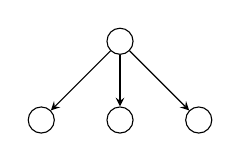
\begin{tikzpicture}[main/.style = {draw, circle}] 
    
        \node[main] (1) {$$}; 
        \node[main] (2) [below of=1] {$ $};
        \node[main] (3) [left of=2] {$$}; 
        \node[main] (4) [right of=2] {$$};
        
        %\draw  node[fill,circle,scale=0.3]{} (0,0);
    
        \draw[-stealth] (1) -- (2);
        \draw[-stealth] (1) -- (3);
        \draw[-stealth] (1) -- (4);  
    \end{tikzpicture} 
\end{center}
Si l'on fixe $\varphi(\delta,t) = \mathds{1}(\delta)_{\llbracket -1, 1\rrbracket}$, alors la dynamique associée est la suivante : si un site $(x,t)$ est à hauteur $\omega(x,t)\geq \sigma_t = 3$ alors ce site distribue un grain à ses voisins $(x+\delta,t+1)$ pour $\delta\in \{-1,0,1\}$.
\end{exmp}
\subsubsection{Normalisation}
Dans toute la suite, on considère $\varphi$ normalisée, quitte à poser $\varphi(., t) = \varphi(., t)/\sigma_{t+1}$, et $\sigma_t = \sigma_t/\sigma_{t+1}$. A chaque instant $t$, on a trois cas, 
\begin{itemize}
	\item $\sigma_t < 1$ alors le système tend à se relaxer car à l'instant $t$, le graphe redistribue plus de grains qu'il peut en redistribuer à la ligne $t+1$.
	\item $\sigma_t > 1$ alors le système tend à s'exciter.
	\item $\sigma_t = 1$ alors le système se conserve (dans l'exemple précédent, le système est conservatif).
\end{itemize}
\subsection{Modèle probabiliste}
Etant donné une configuration $\omega$ tirée uniformément parmi l'ensemble des configurations exactement instables qu'en $s=(0,0)\in\mathbb{Z}^d\times\mathbb{N}$, i.e $ \omega \in \Omega_{0} = \{\omega : \forall s\in (\mathbb{Z}^d\times\mathbb{N})\backslash\{(0,0)\}, \omega(s)<\sigma_t, \omega(0, 0) = \sigma_0\}$. 

On note $p:s\in\mathcal{S}\mapsto \mathbb{E}(X(s))$, la quantité (normalisée) de grains qui s'effondrent sur $s$ sachant qu'il y a initialement ($t=0$) effondrement qu'en $0\in\mathbb{Z}^d$. 

%\begin{align*}
%	\forall \delta\in\mathcal{E}, t\in\mathbb{N}, \varphi^*_{\delta,t} = \frac{\varphi(\delta,t)}{s(t+1)}
%\end{align*}


De la relation de récurrence précédente, on obtient une relation identique à celle d'une marche aléatoire partant de $(0,0)$ avec des pas de déplacements $(\delta, +1)$ de poids $\varphi(\delta, t)$ donnée par le théorème suivant
\begin{theorem}

	La quantité moyenne de grains qui se transmettent au sommet $s$ normalisée est donnée par
	\begin{align*}
	\forall s\in\mathcal{S}^*,\,\,\, p(s) = \sum_{\delta\in \mathbb{Z}^d}p(s-(\delta,1))\varphi(\delta,t-1)\end{align*} 
	\begin{proof}
		Soit $\omega \in\Omega_0$, notons \begin{align*}
		\mathcal{A}_t = \{x \in \mathbb{Z}^d : x \textup{ est accessible depuis } 0 \textup{ en un temps } t \textup{ avec des déplacements admissibles}\}\end{align*}
		
		Soit $x\in\mathbb{Z}^d$, on se donne une bijection $i : \mathcal{A}_{t-1} \to \llbracket 1;|\mathcal{A}_{t-1}|\rrbracket$ pour énumérer $\mathcal{A}_{t-1}$ et on définit
		\begin{align*}\forall j\in\llbracket 0;|\mathcal{A}_{t-1}|\rrbracket, \omega_{j,t} = 
			\left \{
\begin{array}{c @{} c}
	\omega_{t} \,\,\,\, \textup{si }j=0 \\
	T_{(i^{-1}(j),t-1)}(\omega_{j-1,t}) \,\,\,\, \textup{si }j\geq 1\\
\end{array}
\right.\end{align*}

Soit $x\in\mathbb{Z}^d$, on décompose l'application de l'opérateur de toppling $\tau$ sur $\omega_{t}$ par les états successifs $(\omega_{j,t})_j$, ainsi l'ordre d'un produit de topplings est selon l'énumération $i$, posons $A_0 = \varnothing$ et $A_k = \{\omega : (\prod_{y\in\mathcal{A}_{t-1} : i(y)\leq k}){T_{(y,t-1)}}(\omega_{t})(x)\geq \sigma_t\}$, alors $A_k$ est l'ensemble des configurations dont l'effondrement sur $x$ des $k$ premiers-sites $y$ (selon l'énumération $i$) fait de $x$ un site instable en $t$. Nous avons
	\begin{align*}
		\{\omega : x\textup{ s'effondre à l'instant } t\} &= \{\omega : \tau(\omega_t)(x)\geq \sigma_t\}\\
								  &=\{\omega : (\prod_{y\in \mathcal{A}_{t-1}} T_{(y,t-1)})(\omega_{t})(x)\geq \sigma_t\}\\
						   %&= \{\omega : (\prod_{y\in\mathcal{A}_{t-1} \cap \mathcal{S}^{-1}(x)}T_{(y,t-1)})(\omega_{t})(x)\geq \sigma_t\}\\
						    &= \bigsqcup_{k=1}^{|\mathcal{A}_{t-1}|}A_k\backslash A_{k-1}
						   %= \bigsqcup_{k=1}^{|\mathcal{A}_{t-1}|}A_k\backslash A_{k-1}  
						 \end{align*}
						 La première égalité s'obtient par définition de $(x,t)$ instable, la seconde égalité est justifiée car seuls les sites $y\in\mathcal{A}_{t-1}$ s'effondre à l'instant $t-1$.


						 Et $A_k\backslash A_{k-1} = \{\omega : \omega_{t}(x)+\sum_{j<k}\varphi(x-i^{-1}(j), t-1)<\sigma_t, \omega_{t}(x)+\sum_{j\leq k}\varphi(x-i^{-1}(j), t-1)\geq \sigma_t\}$, cela car les $k-1$ premiers effondrements ne rendent pas $(x,t)$ instable mais les $k$ premiers, si. Les quantités $\omega_{t}(x)$ étant distribuées uniformément, on a que pour tout $k \in \llbracket1;|\mathcal{A}_{t-1}|\rrbracket$, la contribution moyenne au site $(x,t)$ du $k$-ème effondrements sachant que $(x,t)$ n'est pas instable après les $k-1$ premiers est  

						 \begin{align*}p(i^{-1}(k),t-1)\varphi(x-i^{-1}(k))\end{align*}
					 
						 %Pour le voir, on peut poser pour tout $I\subset \mathbb{Z}^d$, $X_I = \bigcap_{i\in I} \{\omega : A(i,t-1)=1\} \bigcap_{i\notin I}\{\omega : A(i,t-1)=0\}\cap \{\omega : A(i^{-1}(k),t-1)=1\}$. La formule des probabilités totales donne que $\mathbb{P}(A_k\backslash A_{k-1}) = \sum_{I\subset \mathbb{Z}^d}\mathbb{P}(A_k\backslash A_{k-1}|X_I)\mathbb{P}(X_I)$. Comme les quantités $\omega_t(x)$ sont distribuées uniformément, on a $\mathbb{P}(A_{k}\backslash A_{k-1}|X_I)=\varphi(x-i^{-1}(k),t-1)$. De plus, $\sum_{I\subset \mathbb{Z}^d}\mathbb{P}(X_I) = p(\sqcup_{I\subset \mathcal{E}^{-1}(x)} X_I) = p(A(i^{-1}(k),t-1)=1) = p(i^{-1}(k),t-1)$. Ainsi,
						En sommant toutes les contributions, on obtient

						 \begin{align*}
							 p(x,t) = \sum_{y\in \mathbb{Z}^d}p(y, t-1)\varphi(x-y,t-1) = \sum_{\delta\in \mathbb{Z}^d}p(s-(\delta, 1))\varphi(\delta, t-1)
						 \end{align*}
						 %On a en plus montré que $\mathds{E}(A(s)) = \min\{1, p(s)\}$.
	
	%					 Cette démonstration est quelque peu fastidieuse mais l'idée principale est celle qu'on retrouve dans la démonstration que les opérateurs de topplings commutent. 
					 \end{proof}
\end{theorem}
On définit la série génératrice $\tilde{p}(\Theta, t) = \sum_{x\in \mathbb{Z}^d}p(x,t)e^{i x.\Theta}$ et posons $\mathcal{L}(t,\Theta)= \sum_{\delta\in \mathbb{Z}^d} e^{i\delta.\Theta}\varphi(\delta,t-1)$. Nous obtenons 
\begin{align*}
	\tilde{p}(\Theta, t) = \tilde{p}(\Theta, t-1)\mathcal{L}(t,\Theta)
\end{align*}

\begin{exmp}
	L'exemple du graphe précédent donne 
	\begin{align*}
		p(x, t) = \frac{1}{3}\sum_{\delta=-1}^1 p(x+\delta, t-1)\indent \mathcal{L}(t,\theta) = 1/3(1+2\cos(\theta)) \indent \tilde{p}(\theta, t) = 1/3^t(1+2\cos(\theta))^t
	\end{align*}
\end{exmp}
	\begin{lemma}
	Si l'effondrement initial a lieu en $(0,0)$ alors
	\begin{align*}
		\forall s\in S, p(s) = \sum_{\Delta : (E)}  \Psi(\Delta)
	\end{align*}
	où $\Delta = (\delta_i) : (E)$ est la condition $\sum_{i=0}^{t-1}\delta_{i} = x$ et $\Psi(\Delta) = \prod_{i=0}^{t-1}\varphi(\delta_i,i)$.
	\begin{proof}
		Par hypothèse, l'effondrement initial a lieu en $(0,0)$ ainsi $\tilde{p}(\Theta, 0) = 1$. D'après le résultat qui précède, 
		\begin{align*} \tilde{p}(\Theta, t) = \prod_{i=1}^{t}\mathcal{L}(i,\theta) = \sum_{\Delta\in (\mathbb{Z}^d)^{t}} e^{i\Theta.\sum_{i=0}^{t-1} \delta_i}\Psi(\Delta)\end{align*}
			et en appliquant la transformée de Fourier inverse, 
			\begin{align*}
				p(s) &= \frac{1}{(2\pi)^d}\int_{\Theta\in [0,2\pi]^d} e^{-i\Theta.x} \tilde{p}(\Theta, t)\mathrm{d}\Theta = \sum_{\Delta \in (\mathbb{Z}^d)^t} \mathds{1}_{(E)}(\Delta)\Psi(\Delta)
		\end{align*} 
	\end{proof}\end{lemma}
	Dans le cas particulier où la quantité $\varphi=C\mathds{1}_E$, le lemme précédent dit que $p(s) = C^t\textup{Card}\{(\delta_i)\in (E^d)^t : \sum_{i=0}^{t-1}\delta_i=x\}$. %En se restreignant à $d=1$ et au cas où $\varphi^*$ est constante, nous avons le lemme suivant,
	%\begin{lemma}
	%	Notons $(\delta_1, \ldots,\delta_c)$ une énumération de $\mathcal{E}, m=\max \mathcal{|E|}$, posons \begin{align*}
	%	F(X,Y)=\bigg(\sum_{j\geq 0} Y^j\bigg)^c \prod_{i=1}^c \sum_{j\geq 0} X^{(\delta_i+m+1)j} = \frac{1}{(1-Y)^c}\prod_{i=1}^c \frac{1}{1-X^{\delta_i+m+1}}\end{align*}
	%	alors
	%	\begin{align*}
	%		\forall (x,t)\in S, p(x,t) = \frac{-t!(tm+x+1)!}{4\pi^2\varphi^{*t}} \oint_{\gamma^2} \frac{F(z_1,z_2)}{z_1^{tm+x+2} z_2^{t+1}}\mathrm{d}z_1\mathrm{d}z_2
	%	\end{align*}
	%	\begin{proof}%Cette relation fait intervenir la quantité $\prod_{\tau=t_0}^{t-1} \sum_{\delta\in \mathcal{E}}e^{i\delta.\Theta}\varphi^*_{\delta,t}$ et l'application de la transformée de Fourier inverse revient à calculer le nombre de chemins de $x'$ à $x$ en un temps $t-t_0$ en utilisant des déplacements admissibles, $\delta\in \mathcal{E}$.
	%	Notons $\mathfrak{W}=\{\Delta\in\mathcal{E}^t : s(\Delta) = x\}$, $\mathfrak{W}' = \{(n_1,\ldots,n_c)\in\mathbb{N}^c : \sum_{i=1}^c n_i\delta_i = x, \sum_{i=1}^c n_i = t\}$, alors $\textup{card}\mathfrak{W}\geq \textup{card}\mathfrak{W}'$. En effet, posons
	%		\begin{align*}
	%			i : \Delta=(\delta_j) \mapsto (|\{j : \delta_j = \delta_i\}|)_{i\in\llbracket 1;c\rrbracket}
	%		\end{align*}
	%		alors $i$ est clairement surjective. Or le coefficient devant $Y^tX^{x+t(m+1)}$
	%	\end{proof}
	%\end{lemma}
\begin{lemma}
	Soit $X\subset \mathbb{Z}^d$, on a $\tilde{p}(\Theta, t|X) = \tilde{p}(\Theta, t)\sum_{x\in X}e^{i\Theta.x}$ i.e $p(s|X)=\sum_{x'\in X}p(x-x',t)$.
	\begin{proof}
		Le résultat du lemme 1.1 étant valable pour $p(s|X)$, il suffit de poser que les sites $x\in X$ s'effondre initialement, i.e $p(x,0) = \mathds{1}_X(x)$ et alors \begin{align*}
			\tilde{p}(\Theta, t|X)&=\tilde{p}(\Theta,t|\{0\})\tilde{p}(\Theta,0|X)\\
					      &=\tilde{p}(\Theta, t)\sum_{x\in X}e^{i\Theta.x}
		\end{align*}
	\end{proof}
\end{lemma}

\begin{lemma}
	%Notons $\mathds{P}(s_x)$, la probabilité $\mathds{P}(A(x,t) = 1)$. En supposant que $p\leq 1$ (par exemple la quantité de grains totales $s(t)$ qui peuvent être communiqués par chaque sommet de la ligne $t-1$ est croissante en $t$), la loi conjointe est à un instant $t$
	Notons $p(s_x\cap s_y)$ la probabilité qu'il y ait un effondrement en $x$ et en $y$ à l'instant $t$, on a
\begin{align*}
	\forall x, y\in \mathbb{Z}^d, t\in\mathbb{N}^*, x\neq y, \\p(s_x \cap s_y) &= \sum_{(\delta_1,\delta_2)\in (\mathbb{Z}^d)^2} p(s_x-(\delta_1, 1) \cap s_y-(\delta_2,1))\varphi(\delta_1,t-1)\varphi(\delta_2,t-1)\label{1}\tag{1}
\end{align*} 
Et initialement, $p((x,0)\cap (y,0)) = A(x,0)A(y,0)$. \begin{proof}
	Comme $p\leq 1$, on sait que $X$ et $A$ coïncident en loi. 
	La démonstration est semblable à celle du premier lemme et on obtient pour un effondrement initial en $(0,0)$, $\tilde{p}(\Theta_1, \Theta_2, t)=\sum_{(\Delta_1,\Delta_2)\in (\mathbb{Z}^d)^t\times(\mathbb{Z}^d)^t} e^{i(\Theta_1.s(\Delta_1)+\Theta_2.s(\Delta_2))} \Psi(\Delta_1)\Psi(\Delta_2)$ où l'on note $s(\Delta) = \sum_{\delta\in \Delta}\delta$ et cela se généralise facilement.
\end{proof}
\end{lemma}

\begin{lemma}
	Le processus respecte l'équation de Chapman-Kolmogorov, 
\begin{align*}
\forall t_2\leq t, \,\,p(s|s') = \sum_{y\in\mathbb{Z}^d}p(s|(y,t_2))p((y,t_2)|s')\end{align*}
Avec la condition initiale, $p((x,t')|(x',t')) = \delta_{x, x'}$.
\end{lemma}

\begin{section}{Le cas où $\varphi(x, t) = 1/(2n+1)\mathds{1}(x)_{\llbracket -n; n\rrbracket}$}
\begin{theorem}
	Si $\varphi(x, t) =1/(2n+1)\mathds{1}(x)_{\llbracket -n,n\rrbracket}$ alors 
	\begin{align*}
	  \frac{1}{C^t} \sum_{x\in\mathbb{Z}}p(x,t) X^{nt+x} = \bigg(\sum_{i=0}^{2n} X^i\bigg)^t\end{align*}
	  \begin{proof}
		  On a $C\mathcal{L}(\theta) = \sum_{\delta=-n}^{n} e^{i\delta \theta} = 1 + 2\sum_{\delta=1}^n \cos \delta t$. En posant $\theta = -i \ln X$, le résultat est obtenu.
		%  \begin{align*}
		%	  \frac{1}{C^t}X^{n t} \tilde{p}(-i \ln{X},t) 
		%	  &= \frac{1}{C^t}\sum_{x\in\mathbb{Z}}p(x,t) X^{nt+x}\\
		%						       &= \frac{1}{C^t}X^{n t}\mathcal{L}(-i \ln{X})^t\\
		%	  			      &=X^{n t}\bigg(1+2\sum_{\delta=1}^n \cos\{i \ln{X^{\delta}}\}\bigg)^t\\
		%	  			      &=X^{n t}\bigg(1+\sum_{\delta=1}^n \frac{1+X^{2\delta}}{X^{\delta}}\bigg)^t\\
		%				      &=\bigg(\frac{X^{2n+1}-1}{X-1}\bigg)^t
		 % \end{align*}
		  %Si $\mathcal{E}'$ est à une translation prêt $\mathcal{E}=\llbracket -n,n\rrbracket$ alors le théorème reste valable au décalage prêt des exposants.

	  \end{proof}
\end{theorem}
\begin{theorem}
	Dans les conditions précédentes,  
	\begin{align*}
		\sigma^2(t) = \frac{1}{3} n (1+n) t
	\end{align*}
	\begin{proof}
		Notons $P(X) = \sum_{i=0}^{2n} X^i$ et $\begin{pmatrix}t\\j\end{pmatrix}_{2n+1}$ le coefficient en $X^j$ dans $P(X)^t$, par le théorème qui précède, on a
		\begin{align*}
			(2n+1)^t p(j-nt,t) = \begin{pmatrix} t\\j \end{pmatrix}_{2n+1}
		\end{align*}
		Par symétrie, $p(x,t) = p(-x,t)$ et donc $\mathbb{E}(x : (x,t) \textup{ s'effondre}) = \sum_{x=-n t}^{n t} p(x,t) x = 0$.

		Ainsi, \begin{align*}
			\sigma^2(t) = \textup{Var}(x : (x,t) \textup{ s'effondre}) &=\sum_{x=-nt}^{nt} x^2 p(x,t) - \mathbb{E}(x : (x,t) \textup{ s'effondre})^2\\& = \frac{1}{(2n+1)^t} \sum_{j=0}^{2nt} (j-nt)^2 \begin{pmatrix}t\\j\end{pmatrix}_{2n+1} 
		\end{align*}

		Aussi, les identités 4.2 et 4.3 de \cite{h2} sont
		\begin{align*}
			\sum_{j=0}^{2n t} j^2 \begin{pmatrix} t\\j\end{pmatrix}_{2n+1} = \frac{2nt (2n+1)^t}{12} (2n (3t+1)+2) \indent \indent \sum_{j=0}^{2n t} j \begin{pmatrix} t\\j \end{pmatrix}_{2n+1}  = \frac{2 nt (2n+1)^t}{2}
		\end{align*}
		d'où le résultat. Un calcul similaire peut-être mené dans le cas où $\varphi(x,t) = 1/(2n+1)\mathds{1}(x)_{\llbracket[-n,n\rrbracket+\mu}$, la variance est inchangée.
	\end{proof}
\end{theorem}
%\begin{theorem}
%	Dans les mêmes conditions que le théorème précédent et en posant sans perte de généralité $C = \frac{1}{2n+1}$, le cumulatif $C_p(t)$ d'ordre $p\geq 2$ est pour tout $t$, 
%	\begin{align*}
%		C_p(t) = t\frac{B_p}{p}((2n+1)^p-1)
%	\end{align*}
%	où $B_p$ est le $p$-ème nombre de Bernoulli et avec $C_0 = C_1 = 0$. 
%	En particulier, 
%	\begin{align*}
%		\sigma^2(t) = C_2(t) = \frac{n(n+1)t}{3}
%	\end{align*}
%	\begin{proof}
%		En se référant à \cite{h2}, la fonction génératrice des moments associée à la variable aléatoire discrète $X$ de distribution uniforme sur $\{0, \ldots 2n\}$ est 
%		\begin{align*}
%			\mathds{E}(e^{w X}) = \frac{1}{2n+1}\sum_{j=0}^{2n} e^{w j} =\frac{1}{2n+1} \frac{1-e^{(2n+1)w }}{1-e^{w}}
%		\end{align*}
%
%		Posons $Y(t) = \sum_{j=1}^{t} X_i$ où $X_i\sim X$ et les $(X_i)$ sont i.i.d, comme dans \cite{h2}. On définit la fonction génératrice $f_Y$ des cumulants de $Y$ par \begin{align*}
%			f_Y(w) = \ln\mathds{E}e^{Y(t)} = \ln\mathds{E}\prod_{j=1}^{t}X_i = t \ln\mathds{E}X = tf_X(w)
%		\end{align*}
%
%		On définit les cumulants de $X$ $(C_{X,p})$ par\begin{align*}
%			f_X(w) = \sum_{p=0}^{+\infty} \frac{C_{X,p}}{p!}w^p
%		\end{align*}
%
%		l'égalité $f_Y(w) = tf_X(w)$ implique que 
%		\begin{align*}
%			C_{Y(t),p} = tC_{X,p}
%		\end{align*}
%
%		Le calcul de $C_{X,p}$ pour $p\geq 2$ est mené dans \cite{h3} et cela donne
%		\begin{align*}
%			C_{X,p} = \frac{B_k}{k} ((2n+1)^k-1)
%		\end{align*}
%
%		Pour les deux premiers termes du développement, on a
%		\begin{align*}
%			\lim_{w\to 0} f_X(w) =  0 \indent \lim_{w\to 0} \frac{\mathrm{d}f_X}{\mathrm{d}w}(w) = nt
%		\end{align*}
%
%		Posons $A(t) = A(.,t)$, alors d'après l'égalité utilisée dans le théorème 1.7 et \cite{h2}, \begin{align*}
%			A(t) = Y(t)-nt
%		\end{align*}
%
%		Ainsi, \begin{align*}
%		f_{A(t)}(w) &= \ln\mathds{E}e^{(Y(t)-nt)w}\\
%				    &= -nt w + f_{Y(t)}(w)\\
%				    &= -ntw+tf_X(w)\\
%				    &= t \sum_{p=2}^{+\infty} \frac{C_{X,p}}{p!}w^p\\
%				    &= t \sum_{p=2}^{+\infty} ((2n+1)^p-1)\frac{B_p}{p! p}w^p\end{align*}
%
%	\end{proof}
%\end{theorem}
\begin{theorem}
	Si $\varphi(x,t) = 1/(2n+1)\mathds{1}(x)_{\llbracket -n,n\rrbracket+\mu}$ alors
	\begin{align*}
		X(t) \underset{t\to \infty}{\overset{\mathcal{L}}{\to}} \mathcal{N}(\mu t, \sigma(t)^2 = \frac{1}{3}tn(n+1))
	\end{align*}
	\begin{proof}
		Nous pouvons supposer que $\varphi(x,t)_{\llbracket -n,n\rrbracket}$, le théorème précédent nous dit que si $A(t)$ suit une loi normale de variance $\sigma^2(t)$ alors nécessairement 
	\begin{align*}
		\mu = C_1(t) = 0 \indent C_2(t) = \sigma^2(t)  = \frac{n(n+1)t}{3}
	\end{align*}

	On va utiliser le théorème centrale-limite sur les $(X_i)$ qui sont i.i.d suivant $X$ une variable aléatoire discrète uniforme sur $\llbracket -n,n\rrbracket$. L'expression donnée de $p$ dans le théorème 2.2, $(2n+1)^tp(j-nt,t) = \begin{pmatrix} t\\j\end{pmatrix}_{2n+1}$ ainsi que le théorème 2.1 de \cite{h2} montrent que 
	\begin{align*}
		X(t) = \sum_{i=1}^t X_i - n t
	\end{align*}
	Le théorème centrale-limite donne le résultat, la variance peut être obtenue en utilisant l'expression de la variance de $X$ et l'équation précédente. Il est à noter que le papier \cite{10.2307/1426526} présente un théorème centrale limite pour les marches aléatoires embranchantes à milieux variales. Ce théorème s'applique dans ce cadre et est plus général que le résultat ainsi démontré.
\end{proof}
	
\end{theorem}
\begin{theorem}
	Si $\varphi(x,t) =1/(2n+1) \mathds{1}(x)_{\llbracket -n,n\rrbracket}$ alors
	\begin{align*}
		p(x,t) = t/(2n+1)^t\sum_{p=0}^{\lfloor (x+nt)/(2n+1)\rfloor} \frac{(-1)^p\Gamma(t+x+nt-p(2n+1))}{\Gamma(p+1)\Gamma(t-p+1)\Gamma(x+nt-p(2n+1)+1)}
	\end{align*}
	\begin{proof}
		Pour l'expression de $p$, voir 2.8 de \cite{h2} donnant l'expression de $\begin{pmatrix} t\\j\end{pmatrix}_{2n+1}$. 
	\end{proof}
\end{theorem}
\begin{theorem}
	Si $\varphi(x,t) = 1/(2n+1)\mathds{1}(x)_{k\llbracket -n,n\rrbracket+\mu}$ pour un certain $k\geq 1$ alors
	\begin{align*}
		p(x,t) \underset{t\to \infty}{\to} \frac{1}{\sqrt{2\pi}\sigma(t)} e^{-\frac{(x-\mu t)^2}{2k^2\sigma(t)^2}}\mathds{1}_{k\mathbb{Z}}(x-\mu t) 
	\end{align*}

	où $\sigma(t)^2 = 1/3n(n+1)t$.
	\begin{proof}
		Supposons, sans perte de généralité que $\mu = 0$. D'après le lemme 1.2, on a pour tout $s\in \mathcal{S}$, 
		\begin{align*}
		²p(s) = C^t\textup{Card}\{\{\delta_i\} \in \llbracket -n,n\rrbracket : k\sum_{i=0}^{t-1}\delta_i = x\}
		\end{align*}

		Si $x$ n'est pas divise par $k$, alors $p(s) = 0$. Sinon, $p(s) = C^t\textup{Card}\{\{\delta_i\}\in\llbracket -n,n\rrbracket : \sum_{i=0}^{t-1}\delta_i = x/k\}$. D'après le théorème 2.3, on a le résultat.
	\end{proof}
\end{theorem}
\end{section}
\section{Flux carré moyen}
Le flux carré moyen $\Phi$ est défini par 
\begin{align*}
	\forall t, \Phi(t) = \mathbb{E}\bigg(\sum_{x\in\mathbb{Z}^d}A(s_x)\bigg)^2 
	%= \sum_{(x,y)\in\mathbb{Z}^d\times\mathbb{Z}^d}p(s_x\cap s_y)
\end{align*}

\begin{theorem}
	En dimension $d=1$, supposons que $\varphi$ ne dépend pas de $t$
	%\end{enmerate}
	alors \begin{align*}
		\Phi(t) \sim \frac{1}{\gamma}\sqrt{\frac{t}{\pi}}
	\end{align*}
	où $\gamma$ est défini dans la démonstration.
	\begin{proof}
		Comme $\varphi$ ne dépend pas de $t$, on a que $X$ et $A$ coïncident en loi puis \begin{align*}
			\Phi(t) = \sum_{(x,y)\in\mathbb{Z}^d\times\mathbb{Z}^d} p(s_x \cap s_y)
		\end{align*}

		L'équation linéaire \eqref{1} que respecte la loi conjointe sur une même ligne $t$ a pour solution, pour une certaine fonction $f$, 
\begin{align*}
	p(s_x\cap s_y) = \sum_{Z\in \mathcal{S}} f(Z) p(s_x|Z)p(s_y|Z)
\end{align*}
Définissons $F(t) = \sum_{x\in\mathbb{Z}^d}f(s_x)$. L'hypothèse d'indépendance de $\varphi$ par rapport à $t$ implique qu'il y a conservation du nombre moyen de grains qui se déplacent à chaque instant, donc de $\mathbb{E}\sum_{x\in\mathbb{Z}^d}A(s_x)=\sum_{x\in\mathbb{Z}^d}p(s_x)$. On pose, sans perte de généralité par linéarité, $\sum_{x\in\mathbb{Z}^d}p(s_x) = 1$.

Nous obtenons en utilisant ce qui précède,
\begin{align*}
	\Phi(t) = \sum_{(x,y)\in\mathbb{Z}^d\times\mathbb{Z}^d}\sum_{Z\in S} f(Z)p(s_x|Z)p(s_y|Z) = \sum_{t'=0}^t F(t')
\end{align*}

Posons $K(t) = \sum_{x\in\mathbb{Z}^d} p(s_x)^2$, $\tilde{F}(z) = \sum_{t\in \mathbb{N}}F(t) z^t$ et $\tilde{K}$ les séries génératrices associées. L'hypothèse d'indépendance de $\varphi$ par rapport au temps implique $p(s|s')=p(s-s')$ puis
\begin{align*}
	1 = \sum_{x\in\mathbb{Z}^d}p(s_x) = \sum_{x\in\mathbb{Z}^d, Z\in S}f(Z)p(s_x|Z)^2 = \sum_{t'=0}^t F(t')K(t-t')
\end{align*}

Sur les fonctions génératrices,
\begin{align*}
	\tilde{K}(z)\tilde{F}(z) = \frac{1}{1-z} \tag{2}
\end{align*}

Il ne reste plus qu'à calculer $K(t)$. Si la distribution admet une symétrie par rapport à $0_d$, c'est-à-dire $\varphi(-\delta) = \varphi(\delta)$ alors l'équation de Chapman-Kolmogorov donne $p(0,2t) = K(t)$. 


Plus généralement,
	\begin{align*}
		|\mathcal{L}(\Theta)|^{2t}\tilde{p}(\Theta,0) = \sum_{(x,y)\in\mathbb{Z}^d\times\mathbb{Z}^d} e^{i\Theta.(x-y)}p(s_x)p(s_y)
	\end{align*}

	d'où, 
\begin{align*}
	K(t) = \sum_{x\in \mathbb{Z}}p(s_x)^2 = \frac{1}{(2\pi)^d}\int_{[0,2\pi]^d}|\mathcal{L}(\Theta)|^{2t} \tilde{p}(\Theta, 0)\mathrm{d}\Theta
	\end{align*}

Ainsi, 
\begin{align*}
	\tilde{K}(z)
	%&=\frac{1}{(2\pi)^d}\int_{[0,2\pi]^d}\tilde{p}(\Theta,0)\mathrm{d}\Theta\sum_{t=0}^{+\infty} (z|\mathcal{L}(\Theta)|^2)^t\\
		     =\frac{1}{(2\pi)^d}\int_{[0,2\pi]^d}\frac{\mathrm{d}\Theta}{1-z|\mathcal{L}(\Theta)|^{2}}\tilde{p}(\Theta, 0)
\end{align*}

Supposons que $d=1$, posons $c_2 = \sum_{\delta_1<\delta_2} (\delta_1-\delta_2)^2 \varphi(\delta_1)\varphi(\delta_2)^*$ alors
\begin{align*}
|\mathcal{L}(\theta)|^2 %= \sum_{(\delta_1,\delta_2)\in\mathcal{E}^2} \varphi^*_{\delta_1}\varphi^*_{\delta_2} e^{i\theta(\delta_1-\delta_2)}
			%&= 2\sum_{\delta_1<\delta_2} \varphi^*_{\delta_1}\varphi^*_{\delta_2}\cos(\theta(\delta_2-\delta_1)) + \sum_{\delta\in \mathcal{E}}(\varphi^*_{\delta})^2\\
			= 1-c_2\theta^2+o(\theta^4)
\end{align*}

Où la dernière ligne est obtenue en effectuant un développement limité de $\cos$ et la constante est bien $c_1 = \sum_{\delta_1,\delta_2\in\mathbb{Z}}\varphi(\delta_1)\varphi(\delta_2) = 1\times 1$ par normalisation et indépendance de $\varphi$ par rapport à $t$.

Il s'agit d'obtenir un équivalent de $\tilde{K}$ lorsque $z\to 1^-$. Sans perte de généralité, prenons $\tilde{p}(\Theta,0) = 1$. Soit $\varepsilon > 0$ suffisamment petit, pour $z$ au voisinage de $1$, 
\begin{align*}
	\tilde{K}(z) = \frac{1}{\pi}\int_{0}^{\pi}\frac{\mathrm{d}\theta}{1-z|\mathcal{L}(\theta)|^2} 
	%\sim \frac{1}{\pi}\int_{0}^{\varepsilon} \frac{\mathrm{d}\theta}{1-z|\mathcal{L}(\theta)|^2}
	\sim\frac{1}{\pi}\int_{0}^{\varepsilon}\frac{\mathrm{d}\theta}{1-z(1-c_2\theta^2)} 
\end{align*}

La première égalité est justifiée par $|\mathcal{L}(\theta)|^2 = |\mathcal{L}(2\pi-\theta)|^2$. La première équivalence est justifiée car les deux seuls pôles de la fonction qu'on intègre quand $z\mapsto 1^{-}$ sont $\{0,2\pi\}$.
De plus,
\begin{align*}
	\frac{1}{\pi}\int_{0}^{\varepsilon}\frac{\mathrm{d}\theta}{1-z(1-c_2\theta^2)} = \frac{1}{\pi}\frac{\arctan\varepsilon\sqrt{\frac{c_2 z}{1-z}}}{\sqrt{c_2 z (1-z)}} \sim \frac{1}{2\sqrt{c_2}}\frac{1}{\sqrt{1-z}} = \frac{2\gamma}{\sqrt{1-z}}
\end{align*}

Ainsi, \begin{align*}
	\Phi(t) = \sum_{t'=0}^t \bigg(\frac{1}{(1-z)\tilde{K}(z)}\bigg)_{t'} \sim \frac{1}{2\gamma} \sum_{t'=0}^t \bigg(\frac{1}{\sqrt{1-z}}\bigg)_{t'}
\end{align*}

En utilisant les deux identités suivantes \begin{align*}
	\frac{1}{\sqrt{1-z}} = \sum_{t'=0}^{+\infty} z^t \begin{pmatrix}-1/2 \\ t'\end{pmatrix}(-1)^{t'} \indent \sum_{t'=0}^t \begin{pmatrix}-1/2\\t'\end{pmatrix} (-1)^{t'} = \frac{2}{\sqrt{\pi}} \frac{(1+t)\Gamma(1/2(3+2t))}{\Gamma(2+t)} \sim 2\sqrt{\frac{t}{\pi}}
\end{align*}

On obtient \begin{align*}
	\Phi(t) \sim \frac{1}{\gamma}\sqrt{\frac{t}{\pi}} 
\end{align*}
%Si $E=\{-n,n\}$, un calcul donne avec $a(z) = (\varphi^*_n-\varphi^*_{-n})^2z-(\varphi^*_{n}+\varphi^*_{-n})^2\sim -4\varphi^*_{n}\varphi^*_{-n}$
%\begin{align*}
%	\tilde{K}(z)&\sim \frac{1}{2\pi}\frac{\textup{arccot}{((\varphi^*_{n}+\varphi^*_{-n})\sqrt{(z-1)/a(z)}\varepsilon)}}{n(\varphi^*_{n}+\varphi^*_{-n})\sqrt{a(z)(z-1)}}
%	\sim \frac{1}{4n\sqrt{1-z}\sqrt{\varphi^*_{n}\varphi^*_{-n}}(\varphi^*_{n}+\varphi^*_{-n})} = \frac{2\gamma}{\sqrt{1-z}}
%				\end{align*}

%				Sinon, posons $c_1 = \sum_{\delta_1,\delta_2}  \varphi^*_{\delta_1}\varphi^*_{\delta_2}$, $c_2 = \sum_{\varphi_1>\varphi_2}\varphi^*_{\delta_1}\varphi^*_{\delta_2}(\delta_1-\delta_2)^2$, un développement de l'expression précédente donne 
%			\begin{align*}
%				\tilde{K}(z) \sim \frac{1}{2\pi}\frac{2}{c_2z}\sqrt{\frac{c_2z}{c_1(1-z)}}\textup{arctan}{\sqrt{\frac{c_2z}{c_1(1-z)}}} \sim \frac{1}{2\sqrt{c_2c_1(1-z)}} = \frac{2\gamma}{\sqrt{1-z}}
%			\end{align*}

%			On note $2\gamma$ la constante intervenant devant $(1-z)^{-1/2}$ dans $\tilde{K}(z)$. Ainsi, 
%			\begin{align*}
%				\Phi(t) \sim\frac{1}{2\gamma} \sum_{t'=0}^t \bigg(\frac{1}{\sqrt{1-z}}\bigg)_{t'} \sim \frac{1}{\gamma\sqrt{\pi}} \frac{(1+t)\Gamma(1/2(3+2t))}{\Gamma(2+t)} \sim \frac{1}{\gamma}\sqrt{\frac{t}{\pi}}
%			\end{align*}
Si $\varphi=1/(2n+1)\mathds{1}_{\llbracket-n,n\rrbracket}$, on a $c_1=1$ et $c_2=1/3 n(n+1)$ puis 
\begin{align*}
	\gamma=\frac{\sqrt{3}}{4\sqrt{n(1+n)}}
\end{align*}

et pour $t$ grand, 
\begin{align*}
	\Phi(t) \sim 4\sqrt{\frac{tn(n+1)}{3\pi}}
\end{align*} 

De plus, par rapport au théorème 1.7, on remarque que $\sigma(t) = \sigma(x : (x,t) \textup{ s'effondre})$ et $\Phi(t)$ sont proportionnels pour $t$ grand et le facteur de proportionnalité est $\frac{4}{\sqrt{\pi}}$ i.e \begin{align*}
			\Phi(t) \sim \frac{4}{\sqrt{\pi}} \sigma(t)\end{align*}
		\end{proof}\end{theorem}
		\begin{exmp}
			Dans le cas du graphe initialement traité par Dhar dans \cite{DHARBIS} qui nous sert d'exemple,
			\begin{align*}
			\varphi = 1/3\mathds{1}_{\llbracket -1, 1\rrbracket}, \indent \Phi(t) \sim \sqrt{\frac{32 t}{3\pi}}\end{align*}
		\end{exmp}
Dans les conditions du théorème précédent,
		\begin{lemma}
			\begin{align*}
			F(t) \sim \frac{1}{2\gamma \sqrt{t \pi}}\end{align*}
		\begin{proof}
		En reprenant la démonstration du théorème précédent, on obtient \begin{align*}
			F(t) = \sum_{x\in\mathbb{Z}}f(x,t) \sim \frac{1}{2\gamma}\begin{pmatrix}-1/2\\t\end{pmatrix}(-1)^t
		\end{align*}

		D'où le résultat.
	\end{proof}
\end{lemma}
\section{Généralisations du modèle}
\subsection{Généralisation à une mesure quelconque}
Remarquons que $p(.,t-1)$ est défini par un produit de convolution de $p(.,t-1)$ avec une certaine mesure qui dépend de $t$. Donnons-nous une collection $(\mu_t)_{t\in\mathbb{N}^*}$ de mesures finies sur les boréliens de $\mathbb{R}$ de la forme  
\begin{align*}
	\mathrm{d}\mu_t(y) = g_t(y)\mathrm{d}y
\end{align*}

où $g_t$ est une fonction quelconque intégrable. On définit $\mathfrak{s}_t$ par
\begin{align}
	\mathfrak{s}_t(f)(x) =\int f(x-y)\mathrm{d}\mu_t(y)
\end{align}

où $f$ est une fonction $\mu_t$-intégrale quelconque. On définit $\mathfrak{s}_0(f) = f$. On définit par récurrence, 

\begin{align*}
	\Phi(f)(t)(x) &= \mathfrak{s}_t(\Phi(f)(t-1))(x)\\
		      &=\int \Phi(f)(t-1)(x-y_t)\mathrm{d}\mu_t(y_t)\\
		      &=\int \ldots \bigg(\int f(x-\sum_{j=1}^t y_j) \mathrm{d}\mu_1(y_1)\bigg)\ldots \mathrm{d}\mu_t(y_t)
\end{align*}

\begin{lemma}
	On note $p(x,t) = p(t)(x)$ et  $A(0)$ est le profil initial de l'avalanche en $t=0$, on a alors $p(t)(x) = \Phi(A(0))(t)(x)$ pour $t\geq 1$, en posant pour $t\geq 1$
	\begin{align*}
		g_t(y) = \sum_{\delta \in \mathbb{Z}}\varphi(t-1,\delta)\delta'(y-\delta)
	\end{align*}

	où $\delta'$ est compris comme la limite de la suite des dérivées d'une famille naissante de Dirac. 
	\begin{proof}
		Posons $g_t$ comme dans l'énoncé. Montrons que $p(t) = \mathfrak{s}_t(p(t-1))$ et par récurrence, on aura le résultat. Soit $x\in\mathbb{R}$,  
		\begin{align*}
			\mathfrak{s}_t(p(t-1))(x) &= \int_{y\in\mathbb{R}}\mathrm{d}\mu_t(y)p(t-1)(x-y)\\
						  &= \int_{y\in\mathbb{R}} g_t(y)p(t-1)(x-y)\mathrm{d}y\\
						  &= \int_{y\in\mathbb{R}} \bigg [\sum_{d\in \mathcal{E}}\delta'(y-d)\varphi(t-1,d)\bigg]p(t-1)(x-y)\mathrm{d}y\\
						  &= \sum_{d\in\mathbb{Z}}\varphi(t-1,d) \int_{y\in\mathbb{R}}\delta'(y-d) p(t-1)(x-y)\mathrm{d}y\\
						  &= \sum_{d\in\mathbb{Z}}\varphi(t-1,d) p(t-1)(x-d) \\
						  &= p(t)(x)
		\end{align*}

		La somme est finie, l'interversion somme-intégrable est donc justifiée, la dernière égalité est donnée par le théorème 1.1. L'initialisation est bien vérifiée car $p(0) = A(0)$.
		%\begin{align*}
		%	\mathbb{E}(A(t))(x)) = 
		%\end{align*}

	\end{proof}
\end{lemma}
\begin{lemma}
	Etant donné $p(0)$ un profil initial, et $(\mu_t)$ une collection de mesures finies. On définit $p(t) = \Phi(p(0))(t)$ et on note $\mathcal{L}(\theta,t) = \int_{y\in\mathbb{R}}e^{iy \theta}g_t(y)\mathrm{d}y$ et on définit $\tilde{p}(\theta, t) = \int_{x\in\mathbb{R}} e^{i x \theta} p(t)(x)\mathrm{d}x$ alors 
	\begin{align*}
		\tilde{p}(\theta, t) = \mathcal{L}(\theta, t) \tilde{p}(\theta, t-1)
	\end{align*}

	C'est le pendant des lemmes 1.2 et 1.3.
	\begin{proof}
		Soit $t\in \mathbb{N}^*$, on a formellement
		\begin{align*}
			\tilde{p}(\theta, t) = &\int_{x\in\mathbb{R}}e^{ix\theta}\int_{y\in\mathbb{R}} g_t(y)p(t-1)(x-y)\mathrm{d}y\mathrm{d}x\\
			&= \tilde{p}(\theta, t-1)\int_{y\in\mathbb{R}}e^{iy\theta}g_t(y)\mathrm{d}y\\
			&= \tilde{p}(\theta, 0) \int_{y\in\mathbb{R}^t}e^{i\theta(y_1+\ldots+y_t)}\times\bigg(\underbrace{\prod_{j=1}^t g_j(y_j)}_{=\mathcal{P}(y) \textup{ poids du chemin } (y_1,\ldots, y_t)}\bigg)\mathrm{d}y
		\end{align*}

		Où les interversions des intégrales sont justifiées par le théorème de Fubini-Lebesgue ($\mu_t$ est une mesure finie). Nous sommes à deux doigts d'arriver à une intégrale de chemin... Ainsi,  
		\begin{align*}
			p(t)(x) &= \frac{1}{(2\pi)^t}\int_{y\in\mathbb{R}^t}e^{i\theta (y.\mathds{1}-x)}\tilde{p}(\theta, 0)\mathcal{P}(y) \mathrm{d}y\\
		\end{align*}

		On pose $\tilde{p}(\theta, 0)=1$, alors
		\begin{align*}
			p(t)(x) = \int_{y\in\mathbb{R}^t}\mathds{1}_{y.\mathds{1}=x} \mathcal{P}(y)\mathrm{d}y
		\end{align*}

		Ainsi, si $\tilde{p}(\theta, 0) = \int p(x,0)e^{i x \theta}\mathrm{d}x$ alors 
		\begin{align*}
			p(t)(x) = \int_{z\in\mathbb{R}} p(0)(z)\int_{y\in\mathbb{R}^t}\mathds{1}_{y.\mathds{1}=x-z}\mathcal{P}(y)\mathrm{d}y\mathrm{d}z
		\end{align*}

		Dans le cas précédent, on a $\tilde{p}(\theta, 0) = \sum_{x\in\mathbb{R}}e^{ix \theta}p(x,0)$, ainsi pour passer d'une transforation de Fourier discrète à une transformation de Fourier continue, on remplace $p(0)(x)$ dans $\tilde{p}(\theta, 0) = \int p(0)(x)e^{ix\theta}\mathrm{d}x$ par $p(x,0)g_0(x)$ avec $g_0(x) = \sum_{d}\delta'(x-d)p(d,0)$. Soit $(y_1,\ldots,y_t)$ un chemin, on a dans ce cas
		\begin{align*}
			\mathcal{P}(y) = \prod_{j=1}^t g_j(y_j) = \prod_{j=1}^t \varphi(j-1,y_j)
		\end{align*}

		Et l'on retrouve le résultat les lemmes 1.2 et 1.3.
	\end{proof}
\end{lemma}
\subsection{Passage en temps continu}
On exploite le lemme 4.2 pour nous ramener à une intégrale de chemin. Notons $g_t(y) = g(t,y)$. Soit $y : \mathbb{R}\to \mathbb{R}$ un chemin. On définit alors le poids du chemin $y$ par \begin{align*}
	\mathcal{P}(y) = \exp\{\int_{0}^t \ln g(t, \dot{y}(t))\mathrm{d}t\}
\end{align*}
alors en utilisant la notation des intégrales de chemin de Feynman,
\begin{align*}
	\tilde{p}(\theta, t) = \tilde{p}(\theta, 0)\int e^{i\theta (y(t)-y(0))}\mathcal{P}(y)\mathcal{D}y
\end{align*}

Puis,
\begin{align*}
	p(t)(x) = \int_{z\in\mathbb{R}}p(0)(z)\int_{y(t)-y(0)=x-z} \mathcal{P}(y)\mathcal{D}y\mathrm{d}z
\end{align*}
\section{Temps de relaxation du modèle discret}
\subsection{Temps de relaxation}
%On définit le flux d'ordre $k$ pour $k\geq 1$ par
%\begin{align*}
%	\Phi_k(t) = \mathds{E}\bigg(\sum_{x\in \mathbb{Z}} A(s_x)\bigg)^k = \sum_{X=(x_1,\ldots,x_k)\in\mathbb{Z}^k}\mathds{P}(s_{x_1}\cap \ldots \cap s_{x_k})
%\end{align*}

Définissons la variable de temps de relaxation, $T = \inf\{t\in \mathbb{N} : \cap_{x\in \mathbb{Z}} [A(s_x) = 0]\}$, étant donné une configuration $\omega$, $T(\omega)$ est le temps d'effondrement.   
\begin{theorem}

Dans le cas où $\varphi$ est indépendante de $t$, d'après \cite{1T1}, pour une certaine constante $C$ connue dépendante de $\varphi$, on a
	\begin{align*}
		\lim_{t\to +\infty} \sqrt{t}\mathds{P}(T>t) = C %2\sum_{n=0}^\infty \Phi_{2n+1}(t)-\Phi_{2n}(t)
\end{align*}
%\begin{proof}
	%On a par la formule du crible 
	%\begin{align*}
	%	\mathds{P}(T>t) &= \mathds{P}(\bigcup_{x\in \mathbb{Z}} s_x)\\
	%			    &= \sum_{\varnothing \neq I \subset \mathbb{Z} : |I|<\infty} (-1)^{|I|-1} \mathds{P}(\bigcap_{i\in I}s_x)\\
	%			    &= 1-(\Phi_2(t)-1)+(\Phi_3(t)-\Phi_2(t))-\ldots\\
	%			    &= 2\sum_{n=0}^{\infty}\Phi_{2n+1}(t)-\Phi_{2n}(t)
	%\end{align*}
%\end{proof}
\end{lemma}
\section{Conjecture sur les flux d'ordre supérieur}
On définit le flux d'ordre $k$ pour $k\geq 1$ par 
\begin{align*}
	\Phi_k(t) = \mathds{E}\bigg(\sum_{x\in\mathbb{Z}} A(s_x)\bigg)^k = \sum_{X=(x_1,\ldots,x_k)\in\mathbb{Z}^k}\mathds{P}(s_{x_1}\cap\ldots\caps_{x_k})
\end{align*}

En reprenant le calcul de $\Phi_2$, on pose par analogie $K_k(t) = \sum_{x\in\mathbb{Z}}p(x,t)^k$. La conjecture (motivée par des résultats numériques) que nous faisons est que
\begin{align*}
	K_k(t) \sim t^{(1-k)/2}/C_k
\end{align*}

pour une certaine constante $C_k$, puis similairement, on obtient $\Phi_k(t) \sim C_k\sum_{t'=0}^t \bigg((1-z)^{(1-k)/2}\bigg)_{t^'}$.

En utilisant $\sum_{t'=0}^t (-1)^{t'}\begin{pmatrix}(1-k)/2\\t'\end{pmatrix} \sim t^{(k-1)/2}C_{2, k}$, on aurait, $\Phi_k(t) \sim C_k C_{2,k}t^{(k-1)/2}$ avec $C_{2, 2k} = 2^k/(2k-1)!!\sqrt{\pi}$ et $C_{2,2k+1}=1/k!$. De manière à ce qu'on ait
\begin{align*}
	\Phi_{2n+1}(t) \sim \frac{C_{2n+1}}{n!}t^{(k-1)/2} \indent \Phi_{2n}(t) \sim \frac{C_{2n}2^n\sqrt{\pi}}{(2n-1)!!} t^{(k-1)/2}
\end{align*}










%\subsection{Passage en temps continu}
%Supposons que $g : (t,y) \mapsto g(t,y)$ est $C^1$. En reprenant l'équation précédente pour des temps continus, on obtient,
%\begin{align*}
%	p(x,t) = \int_{y\in\mathbb{R}} g(t,y) (p(x-y,t)-\frac{\partial p}{\partial t}(x-y,t))\mathrm{d}y
%\end{align*}
%\begin{theorem}
%	En dimension $d=1$, supposons que
%	\begin{itemize}
%		\item $\mathrm{d}\mathbb{P}$ ne dépend pas de $t$
%		\item $c_1 = \iint \mathrm{d}\mathbb{P}(\delta_1) \mathrm{d}\mathbb{P}(\delta_2) = 1$
%	\end{itemize}
%
%	alors \begin{align*}
%		\Phi(t) = \iint \mathrm{d}_{(A_t,A_t)}(x,y) \mathds{1}((A_t(x), A_t(y))=(1,1)) \sim \frac{1}{\gamma}\sqrt{\frac{t}{\pi}}
%	\end{align*}
%	\begin{proof}
%		Tout le raisonnement du théorème précédent est valable et cela en posant \begin{align*}
%			\tilde{p}(\theta, t)=  \int p(x,t)e^{ix\theta}\mathrm{d}x = \tilde{p}(\theta, t-1) \mathcal{L}(t,\theta)
%		\end{align*}
%		avec $\mathcal{L}(t,\theta) = \int e^{i y \theta}\mathrm{d}\mathbb{P}_t(y)$ et $c_2 = \iint_{\delta_1<\delta_2}(\delta_1-\delta_2)^2\mathrm{d}\mathbb{P}(\delta_1)\mathbb{P}(\delta_2)$.


%\end{proof}
%\end{theorem}
%\subsection{Limite en temps continu}
%Notons $\mathfrak{s}_t(f)(x) = f(t,x)$, supposons que $f$ est une fonction de classe $\mathcal{C}^1$ en la première variable. Supposons que $\mathrm{d}\mathbb{P}_t(y) = g(t,y)\mathrm{d}y$ où $g$ est une fonction $\mathcal{C}^1$. L'équation (1) précédente devient, 
%\begin{align*}
%	f(t+\Delta t,x) &= \int f(x-y,t)g(t,y)\mathrm{d}y\\
%			&= f(t,x) + \Delta t \frac{\partial f}{\partial t}(t,x)
%\end{align*}
%\begin{lemma}
%	On sait par le théorème 2.5 que
%	\begin{align*}
%		p(s_x|Z) = p(s_x-Z) \sim \frac{1}{\sqrt{2\pi}\sigma(t-\tau)}e^{-\frac{(x-z)^2}{2\sigma(t-\tau)}}
%	\end{align*}
%\end{lemma}
		%		\begin{lemma}
%			\begin{align*}
%				\forall x,y\in \mathbb{Z}^d, t>1, p((x,t)|(y,t)\cap(0,0)) = 
%			\end{align*}
%			\begin{proof}
%				\begin{align*}
%					p((x,t-1)|(y,t))=\frac{1}{\delta^*_{y-x,t-1}}
%				\end{align*}
%			\end{proof}
%M		\end{lemma}

		%\section{Modèle continu en temps : équation de Chapman-Kolmogorov et équations aux dérivées partielles}

%			On peut dériver l'équation de Chapman-Kolmogorov pour obtenir des équations aux dérivées partielles sur la fonction génératrice $\tilde{p}(\Theta, t | s) = \sum_{x\in \mathbb{Z}^d}e^{i x. \Theta} p((x,t)|s)$, voir \cite{MST}. On suppose $t\mapsto \varphi^*_{\delta,t}$ continue sur $\mathbb{R}^+$ et qui représente la quantité normalisée de grains que fournit $s$ à $s+\delta$ entre $t-\mathrm{d}t$ et $t$, avec donc $\sum_{\delta\in \mathcal{E}}\varphi^*_{\delta,\tau} =\lim_{\mathrm{d}\tau \to 0} S(\tau)/S(\tau-\mathrm{d}\tau) = 1$. La \textit{master equation} du processus est avec $s_0 = (x_0,t_0)$,
%			\begin{align*}
%				\frac{\partial p(x,\tau|s_0)}{\partial \tau} = \sum_{\delta\in \mathcal{E}}\varphi^*_{\delta,\tau} (p(x-\delta, \tau|s_0)-p(x,\tau|s_0))
%			\end{align*}
			
%			cela pour tout $\tau \geq t_0$ et avec pour condition initiale, $p(x,t'|s_0) =\delta_{x,x_0}$. Cela donne pour $\tilde{p}$, 
%			\begin{align*}
%				\frac{\partial \tilde{p}(\Theta, \tau)}{\partial \tau}=\tilde{p}(\Theta,\tau)\sum_{\delta\in \mathcal{E}}\varphi^*_{\delta, \tau}(e^{i\delta.\Theta}-1)
%			\end{align*}

%			avec pour condition initiale, $\tilde{p}(\Theta,t_0|s_0)=e^{ix_0.\Theta}$. Cette équation a pour solution
%			\begin{align*}
%				\tilde{p}(\Theta, t|s_0) = \exp\bigg(\int_{t_0}^{t}\sum_{\delta\in \mathcal{E}} (e^{i\delta.\Theta}-1)\varphi^*_{\delta,\tau}\mathrm{d}\tau\bigg)e^{ix_0.\Theta} = e^{-(t-t_0)}e^{ix_0.\Theta}\exp\bigg(\int_{t_0}^t \sum_{\delta\in \mathcal{E}}e^{i\delta.\Theta}\varphi^*_{\delta,\tau}\mathrm{d}\tau\bigg)
%			\end{align*}

			%En calculant la transformée Fourier inverse, on obtient,
			%\begin{align*}
			%	p(x, \tau|s_0) = \frac{1}{4\pi^2}\int_{[0,2\pi]^2}e^{-i x.\Theta} \tilde{p}(\Theta,t|s_0)\mathrm{d}\Theta
			%\end{align*}

%			Effectuons un développement des exponentielles dans $\tilde{p}(\Theta, t|s_0)$, \begin{align*}
%				e^{t-t_0}\tilde{p}(\Theta,t|s_0) &=e^{ix_0.\Theta} \sum_{k=0}^{+\infty}\frac{1}{k!}\bigg(\sum_{\delta\in \mathcal{E}}\int_{t_0}^te^{i\delta.\Theta}\varphi^*_{\delta,\tau}\mathrm{d}\tau\bigg)^k\\
%								 &=e^{ix_0.\Theta}\sum_{k=0}^{+\infty}\sum_{|\alpha|=k}\frac{1}{\alpha_1!\ldots\alpha_{|\mathcal{E}|}!}\exp(i\Theta.\sum_{\delta_i\in \mathcal{E}}\alpha_i\delta_i)\prod_{\delta_i\in \mathcal{E}} \bigg(\int_{t_0}^t \varphi^*_{\delta_i,\tau}\mathrm{d\tau}\bigg)^{\alpha_i}
%			\end{align*}

%			En appliquant la transformée de Fourier inverse, \begin{align*}
%				e^{t-t_0}p(x,t|s_0) = \sum_{k=0}^{+\infty}\sum_{|\alpha|=k : x_0-x+\sum{\alpha_i\delta_i} = 0} \frac{1}{\alpha_1!\ldots\alpha_{|\mathcal{E}|}!}\prod_{\delta_i\in \mathcal{E}}\bigg(\int_{t_0}^t \varphi^*_{\delta_i,\tau}\mathrm{d}\tau\bigg)^{\alpha_i} 
%\ll			\end{align*}

%			Comme prévu, la somme ne porte que sur l'ensemble des chemins composés de déplacements admissibles $\delta\in E$ partant de $x_0$ arrivant à $x$. 
			%\section{Modèle continu en temps : inégalités et expressions asymptotiques}
			%Si $E\subset \mathbb{Z}$, notons $n=|E|$ et supposons que $0\notin E$, pour $x$ grand
			%	\begin{align*}
			%	&\frac{(x+n-1)!}{x!(n-1)!}\frac{|\textup{Div}(\bigwedge_{\delta\in E}\delta)|}{\prod_{\delta\in E}\delta}\sum_{k\geq x/\max_{\delta\in E}|\delta|} (\lfloor k/n\rfloor !)^{-n}\prod_{\delta\in E}\bigg(\int_{t_0}^t \varphi_{\delta,\tau}^*\mathrm{d}\tau\bigg)^{k/n} \leq e^{t-t_0}p(x,t) \\ &\leq\frac{(x+n-1)!}{x!(n-1)!}\bigg(\frac{1}{\prod_{\delta\in E}\delta} + |\textup{Div}(\bigwedge_{\delta\in E}\delta)|-1\bigg)\sum_{k\geq x/\max_{\delta\in E}{|\delta|}}(\lceil k/n \rceil!)^{-n}\prod_{\delta\in E}\bigg(\int_{t_0}^t \varphi^*_{\delta,\tau}\mathrm{d}\tau\bigg)^{k/n}
			%	\end{align*}
			%\section{Temps d'arrêt d'un effondrement}
			%Considérons qu'initialement, il y a un effondrement qu'en $(0,0)$. Posons $\tau = \mathbb{E}\{t : \textup{temps d'arrêt}\}$
			%\begin{proof}
				%\begin{align*}
				%	\mathbb{E}\{t : \sum_{x\in\mathbb{Z}^d}A(x,t) = 0\} &= \sum_{t=1}^{+\infty} t \mathds{P}(\bigcap_{x\in \mathbb{Z}^d} \{A(x,t) = 0\}) \\
				%							    &= \sum_{t=1}^{\infty} t \mathds{P}(\bigcap_{x\in \mathcal{A}_t}\{A(x,t) = 0\})\\
				%							    &=\sum_{t=1}^{\infty}t\prod_{i = 1}^{|\mathcal{A}_t|-1} \mathds{P}(A(x_{i+1},t)=0 | \bigcap_{1\leq j\leq i} \{A(x_i, t) = 0\})
				%\end{align*}
				%\begin{align*}
				%	\mathbb{E}\{t : \textup{temps d'arrêt}\} &= \sum_{t=0}^{+\infty} \mathds{P}\{\textup{temps d'arrêt} > t\}\\
				%						 &=\sum_{t=0}^{+\infty} \mathds{P}(\bigcup_{x\in \mathcal{A}_t} \{A(x, t) = 1\})\\
				%						 &=\sum_{t=0}^{+\infty}\sum_{\varnothing\neq I\subset \mathcal{A}_{t}} (-1)^{|I|-1} \mathds{P}(\bigcap_{i\in I}\{A(x,t) = 1\})\\
				%						 &=\sum_{t=0}^{+\infty}\sum_{\varnothing\neq I\subset \llbracket 1;|\mathcal{A}_t|\rrbracket} (-1)^{|I|-1} \prod_{i=0}^{|\mathcal{A}_t|-1}\mathds{P}(\{A(x_{i+1},t)=1\}|\bigcap_{1\leq j< i}\{A(x_j,t)=1\}\cap\{A(0,0)=1\})\\
				%					 	&=\sum_{t=0}^{+\infty}\sum_{\varnothing \neq I \subset \mathcal{A}_t} (-1)^{|I|-1} \prod_{i\in I}p(i,t)
				%						\leq\sum_{t=0}^{+\infty} \sum_{x\in \mathcal{A}_t}p(s)
				%\end{align*}
			%\end{proof}
%			\begin{section}{Généralisation du modèle d'une mesure discrète à une mesure continue}
%				Considérons l'espace mesurable $(\mathbb{R}^d, \mathcal{B}(\mathbb{R}^d))$ et posons la mesure 
%				\begin{align*}
%					\mu_t(x) = \sum_{\beta \in \mathcal{E}} \varphi_{\beta, t}^* \delta(x-\beta)
%				\end{align*}

%				alors le Lemme 1 se réecrit 
%				\begin{align*}
%					\forall (x,t)\in \mathcal{S}, p(x,t) = \int p(x-y,t-1)\mathrm{d}\mu_{t-1}(y)
%				\end{align*}

%				Ainsi, une généralisation à un espace continue pour la variable $x \in\mathbb{R}^d$ est le même produit de convolution pour une mesure $\mu_t$ quelconque.
%		\end{section}
%		\begin{section}{Modèle continu en temps et pour une mesure quelconque}
%			Soit $\mu : t \mapsto \mu_t$ où $\mu_t$ est une mesure de probabilité, i.e $\int \mathrm{d}\mu = 1$, la master équation devient 
%			\begin{align*}
%				\frac{\partial p(x,t)}{\partial t} = \int  p(x-y,t)\mathrm{d}\mu_t(y) - p(x,t)
%			\end{align*}
%		\end{section}
			%\section{Questions ouvertes}
			%Calculer les grandeurs suivantes
			%\begin{align*}
			%	\forall I\subset Z^d, \forall n\in \mathbb{N},\forall T\in\mathbb{N}, \mathds{P}(\sum_{x\in I}A(x,t)\geq n), \mathds{P}(\sum_{t=0}^T\sum_{x\in I}A(x,t) = 0)\\
			%	\forall n\in\mathbb{N}, \tau_n = \min\{t\in\llbracket 0; +\infty\rrbracket \sum_{x\in Z^d}A(x,t) = n\}, \mathds{E}\tau_n\\
			%	\forall x\in\mathbb{Z}^d, \forall n\in\mathbb{N}, \forall T\in\mathbb{N}, \mathds{P}(\sum_{\tau = 0}^T A(x,t) \geq n)\\
			%	\forall \varphi, \forall t\in\mathbb{N}, \mathds{E}(\sum_{x\in \mathbb{Z}^d} A(x,t)\\
			%	\forall n\in\mathbb{N}, S_n = \sum_{t=0}^{+\infty}(\sum_{x\in \mathbb{Z}^d}A(x,t))(\omega)\mathds{1}_{t=\tau_n}(\omega), \mathds{E}(S_n^2), \mathds{E}(S_n)\\
			%	\forall T\in\mathbb{N}, \mathds{P}(\sum_{t=0}^T \sum_{x>moy(\mathcal{E})} A(x,t) = 0)\\
			%	\end{align*}
			\bibliographystyle{alpha}
			\bibliography{bs}
			\end{document}
